\documentclass{beamer}

\usepackage[orientation=landscape,size=a0,scale=1.4,debug]{beamerposter}
\mode<presentation>{\usetheme{mlr}}

\usepackage[utf8]{inputenc} % UTF-8
\usepackage[english]{babel} % Language
\usepackage{hyperref} % Hyperlinks
\usepackage{ragged2e} % Text position
\usepackage[export]{adjustbox} % Image position
\usepackage[most]{tcolorbox}
\usepackage{listings} % for R code
\lstset{language=R,
    basicstyle=\small\ttfamily,
    stringstyle=\color{DarkGreen},
    otherkeywords={0,1,2,3,4,5,6,7,8,9},
    morekeywords={TRUE,FALSE},
    deletekeywords={data,frame,length,as,character},
    keywordstyle=\color{blue},
    commentstyle=\color{DarkGreen},
}

\title{mlr3tuning :\,: CHEAT SHEET} % Package title in header, \, adds thin space between ::
\newcommand{\packagedescription}{ % Package description in header
	The \textbf{mlr3tuning} package provides hyperparameter tuning for mlr3.
}

\newlength{\columnheight} % Adjust depending on header height
\setlength{\columnheight}{84cm} 

\newtcolorbox{codebox}{%
	sharp corners,
	leftrule=0pt,
	rightrule=0pt,
	toprule=0pt,
	bottomrule=0pt,
	hbox}

\newtcolorbox{codeboxmultiline}[1][]{%
	sharp corners,
	leftrule=0pt,
	rightrule=0pt,
	toprule=0pt,
	bottomrule=0pt,
	#1}

\begin{document}
\begin{frame}[fragile]{}
	\begin{columns}
		\begin{column}{.245\textwidth}
			\begin{beamercolorbox}[center]{postercolumn}
				\begin{minipage}{.98\textwidth}
					\parbox[t][\columnheight]{\textwidth}{
						\begin{myblock}{Intro}
							The mlr3tuning package is an extension for the \href{https://github.com/mlr-org/mlr3}{mlr3} package and provides R6 classes for hyperparameter tuning.
							\\
							\\
							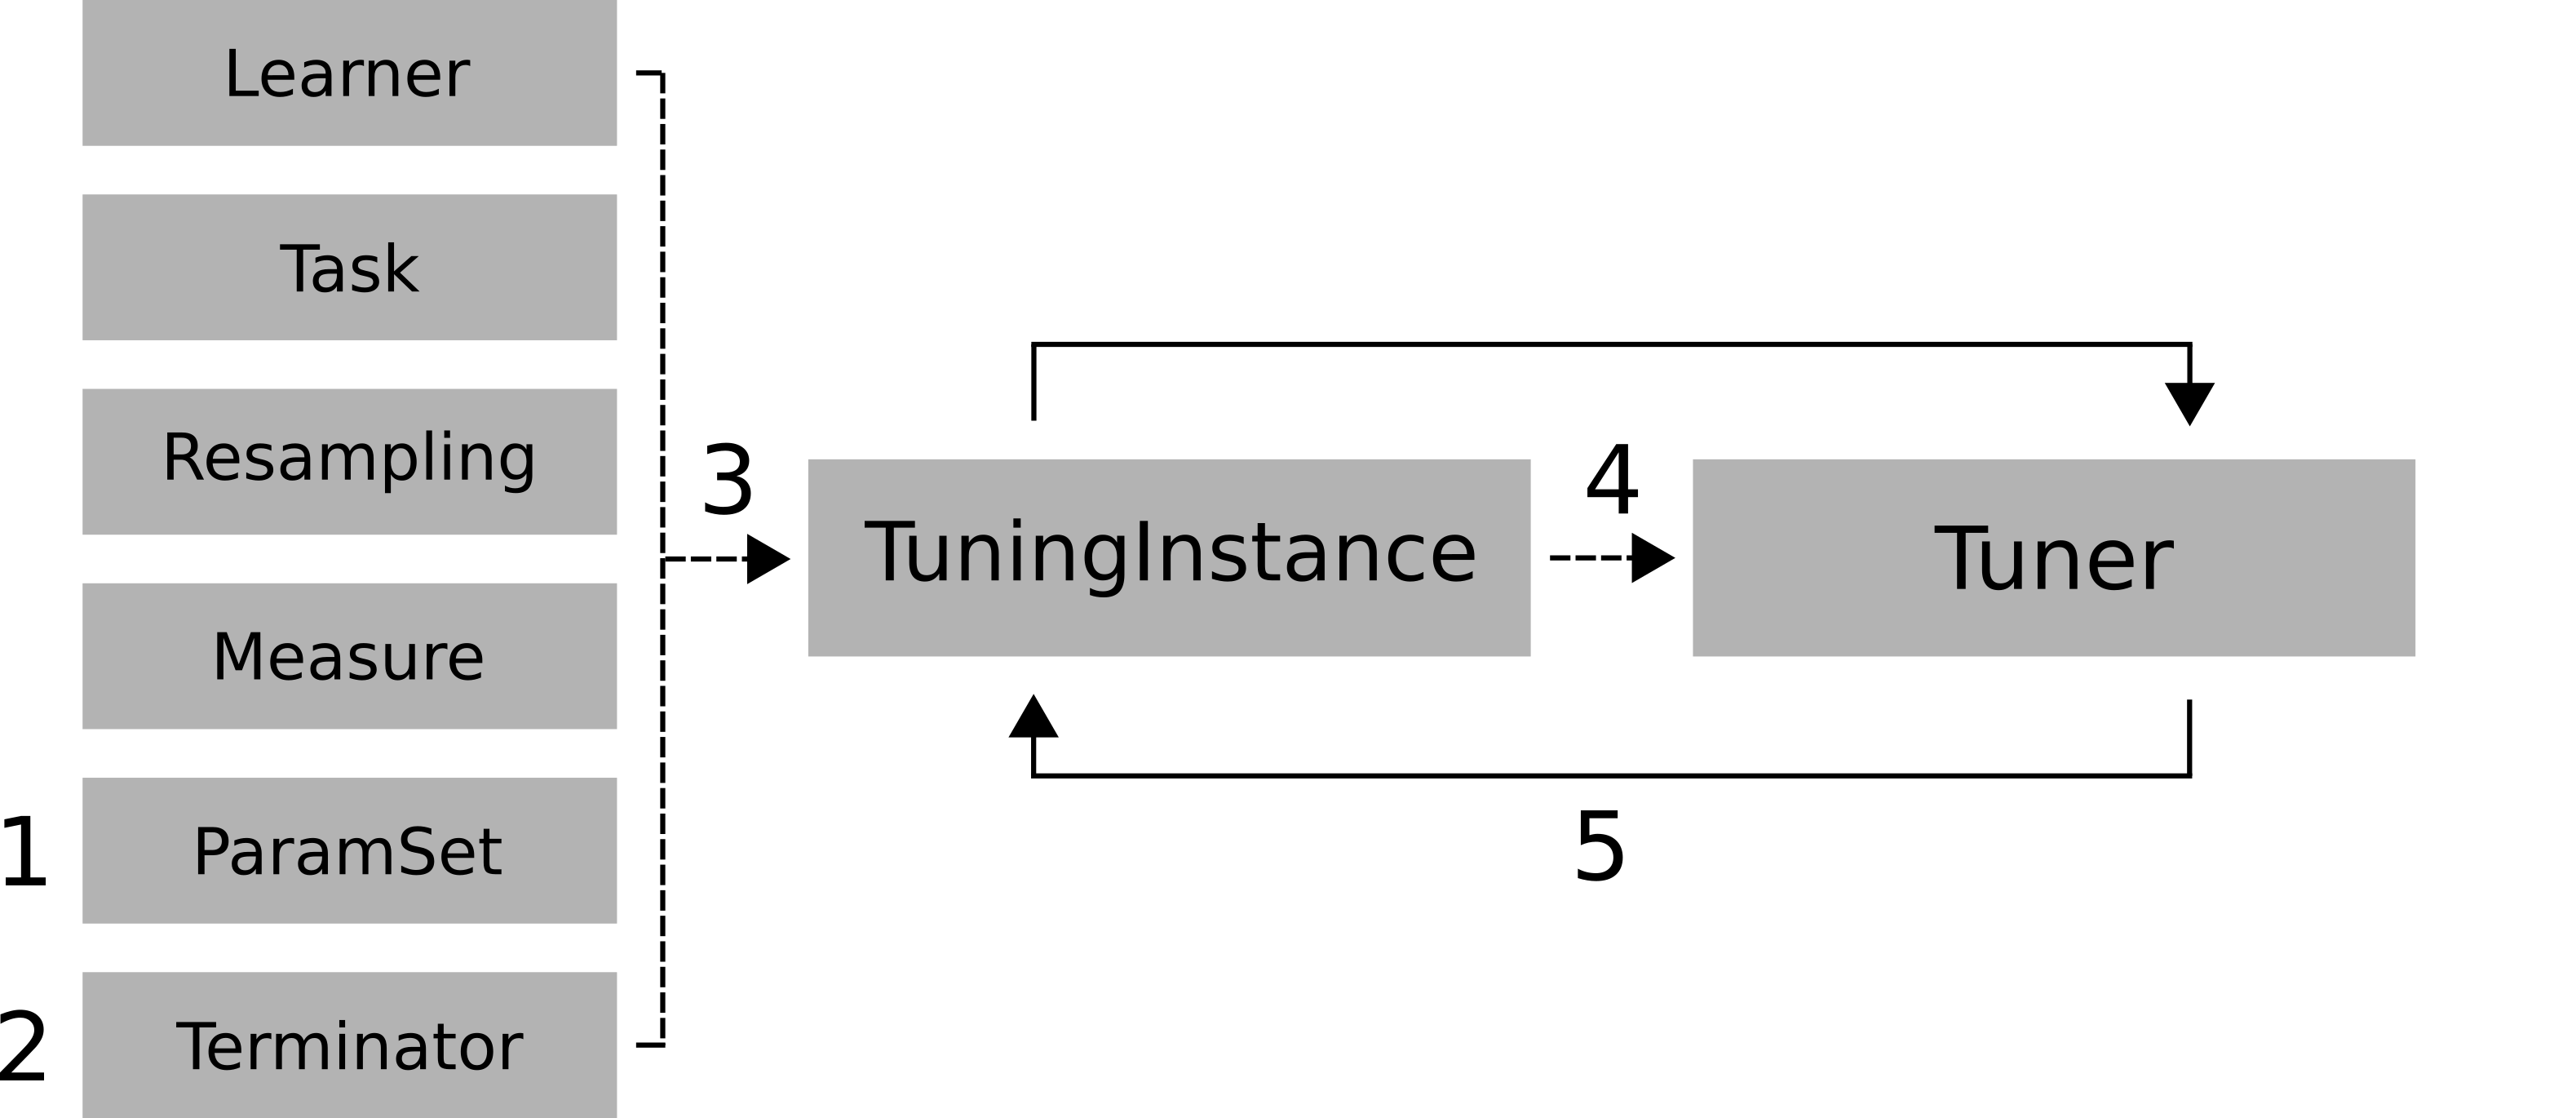
\includegraphics[width=\textwidth]{img/tuning_objects.png}
						\end{myblock}
					\begin{myblock}{Terminator}
						The Terminator determines when to stop the tuning. The package provides four Terminator classes:
						\\
						\begin{codebox}
							terminator = TerminatorClockTime\$new()
						\end{codebox}
						Terminate after a given time 
						\\
						\begin{codebox}
							terminator = TerminatorEvals\$new()
						\end{codebox}
						Terminate after a given amount of iterations 
						\\
						\begin{codebox}
							terminator = TerminatorPerfReached\$new()
						\end{codebox}
						Terminate after a specific performance is reached  
						\\
						\begin{codebox}
							terminator = TerminatorStagnation\$new()
						\end{codebox}
						Terminate when tuning does not improve
						\\
						\begin{codebox}
							terminator = TerminatorCombo\$new()
						\end{codebox}
						A combination of the above in an ALL or ANY fashion
						\\
						\begin{codebox}
							terminator = term(key, ...)
						\end{codebox}
						Get terminator by \textit{key} and construct terminator with settings (...) in one go. 
					\end{myblock}	
					\vfill}
				\end{minipage}
			\end{beamercolorbox}
		\end{column}
		\begin{column}{.245\textwidth}
			\begin{beamercolorbox}[center]{postercolumn}
				\begin{minipage}{.98\textwidth}
					\parbox[t][\columnheight]{\textwidth}{
						\begin{myblock}{ParamterSet}
						The ParamSet defines the hyperparamter to tune and the tuning space.
							\\
							\begin{codeboxmultiline}[width=18cm]
								tune\_ps = ParamSet\$new(list(\\
								\hspace*{1ex}ParamInt\$new(id, lower, upper)\\
								\hspace*{1ex}ParamDbl\$new(id, lower, upper)))
							\end{codeboxmultiline}
					The \textit{id} (character value) refers to the hyperparameter of the learner. The \textit{lower} and \textit{upper} parameter define the bounds of the tuning space. 	
						\end{myblock}	
					\begin{myblock}{TuningInstance}
						The TuningInstance specifies a general search scenario.
						\\
						\begin{codeboxmultiline}[width=18cm]
							instance = \textbf{TuningInstance}\$new(\\
							\hspace*{1ex}task,\\
							\hspace*{1ex}learner,\\
							\hspace*{1ex}resampling,\\
							\hspace*{1ex}param\_set,\\
							\hspace*{1ex}terminator)
						\end{codeboxmultiline}
						The TuningInstance is constructed by supplying a \textit{task}, \textit{learner}, \textit{resampling}, \textit{param\_set} and \textit{terminator}. 
						\\
					\end{myblock}	
					\vfill}
				\end{minipage}
			\end{beamercolorbox}
		\end{column}
		\begin{column}{.245\textwidth}
			\begin{beamercolorbox}[center]{postercolumn}
				\begin{minipage}{.98\textwidth}
					\parbox[t][\columnheight]{\textwidth}{
						\begin{myblock}{Tuner}
							The Tuner describes the tuning strategy. The package provides three algorithms:
							\\
							\begin{codebox}
								tuner = TunerGridSearch\$new()
							\end{codebox}
							Grid search
							\\
							\begin{codebox}
								tuner = TunerRandomSearch\$new()
							\end{codebox}
							Random Search
							\\
							\begin{codebox}
								tuner = TunerGenSA\$new()
							\end{codebox}
							Generalized Simulated Annealing
							\\
							\begin{codebox}
								tuner = trn(key, ...)
							\end{codebox}
							Get tuner by \textit{key} and construct tuner with settings (...) in one go.
						\end{myblock}
					\vfill}
				\end{minipage}
			\end{beamercolorbox}
		\end{column}
		\begin{column}{.245\textwidth}
			\begin{beamercolorbox}[center]{postercolumn}
				\begin{minipage}{.98\textwidth}
					\parbox[t][\columnheight]{\textwidth}{
						\begin{myblock}{Automatic Tuning}
						The AutoTuner wraps a learner and augments it with an automatic tuning for a given set of hyperparameters. 
						\\
						\begin{codeboxmultiline}[width=18cm]
							at = AutoTuner\$new(
\\
							\hspace*{1ex}learner,
\\
							\hspace*{1ex}resampling,
\\
							\hspace*{1ex}measures,
\\
							\hspace*{1ex}tune\_ps,
\\
							\hspace*{1ex}terminator,
\\
							\hspace*{1ex}tuner)
						\end{codeboxmultiline}
						The AutoTuner is constructed by supplying a \textit{task}, \textit{learner}, \textit{resampling}, \textit{param\_set}, \textit{terminator} and \textit{tuner}. 
						\\
						\\
						The AutoTuner inherits from the Learner class and therefore can be used like any other learner.
						\\
						\begin{codebox}
							at\$predict(task, row\_ids)
						\end{codebox}
						Use the tuned Learner in AutoTuner to create a new Prediction.
						\\
						\begin{codebox}
							at\$train(task)
						\end{codebox}
						Train the tuned Learner in AutoTuner on a new Task.
						\end{myblock}
					\vfill}
				\end{minipage}
			\end{beamercolorbox}
		\end{column}
	\end{columns}
\end{frame}
\end{document}
